\section{Hardware and Software Mapping}
As figure \ref{fig:Hardware-Software-Mapping} shows, we want to run the DriveIT subsystems on the following hardware:\\

The Persistence, \texttt{DriveIT Web API} and \texttt{DriveIT Web Client} subsystems will be hosted on a web server running ASP.NET. We have chosen \texttt{Microsoft Azure} as our host.

The \texttt{DriveIT Web API} uses Persistence module internally to contact the \texttt{Microsoft SQL Server} that runs behind the \texttt{Entity Framework}.

The \texttt{DriveIT Web Client} is accessed through a modern web browser using HTTP. It uses the \texttt{DriveIT Web API} internally, and as they are located in the same project, they can be hosted at the same address on \texttt{Microsoft Azure}.\\

The \texttt{DriveIT Windows Client} runs on .NET 4.5 and uses the \texttt{CarQuery} subsystem, which helps \texttt{Employee}s fill out missing information about cars. The \texttt{DriveIT Windows Client} communicates with the \texttt{DriveIT Web API} subsystem through HTTP. The content of the HTTP-requests and responses are Json objects when data transfer is needed.

\begin{figure}[H]
	\centering
	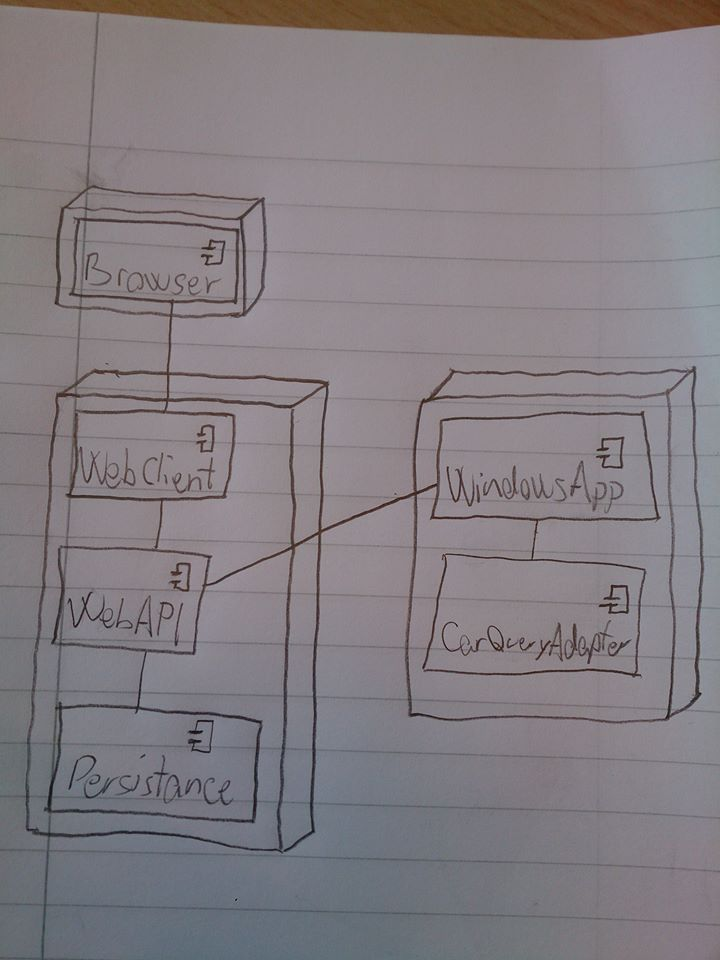
\includegraphics[width=\textwidth]{Figures/HardwareSoftwareMapping}
	\caption{Hardware software mapping of the entire system.}
	\label{fig:Hardware-Software-Mapping}
\end{figure}